\documentclass[../../../../main.tex]{subfiles}
\begin{document}
\section*{京都大学 1980年 前期}
\begin{center}
\begin{tabular}{|c|c|c|c|c|c|}
\hline
\multicolumn{2}{|c|}{} & 計 & 思 & 線 & \\
\hline
\text{\fbox{1}} & 行列 & & & & \\
\hline
\text{\fbox{2}} & 多変数 & A & A & A & 20 \\
\hline
\text{\fbox{3}} & 空間 & B & B & B & 20 \\
\hline
\text{\fbox{4}} & 独立 & A & A & A & 20 \\
\hline
\text{\fbox{5}} & 整数 \textcolor{blue}{A} & A & C & C & 20 \\
\hline
\text{\fbox{6}} & 関数 \textcolor{blue}{A} & B & B & B & 20 \\
\hline
\end{tabular}
\end{center}

\subsection*{第1問}

\subsection*{第2問}
[解] $y=a\left(x+\frac{b}{2a}\right)^2 - \frac{b^2}{4a}$ の頂点 $\left(-\frac{b}{2a}, -\frac{b^2}{4a}\right)$ が
$y=-2x+5$ 上にあるので、
\begin{align*}
-\frac{b^2}{4a} &= \frac{b}{a} + 5 \\
\therefore \quad a &= -\frac{1}{5} \left( \frac{1}{4} b^2 + b \right) \cdots\text{①}
\end{align*}
又、題意の面積 $S$ として ① から
\begin{align*}
S &= \int_{0}^{-\frac{b}{a}} (ax^2 + bx) \,dx \\
&= -\frac{a}{6} \left(-\frac{b}{a}\right)^3 = \frac{1}{6} \frac{b^3}{a^2} \\
&= \frac{1}{6} \frac{b^3}{\frac{1}{25} b^2\left(\frac{1}{4}b+1\right)^2} = \frac{25}{6} \frac{b}{\left(\frac{1}{4}b+1\right)^2} \\
&= \frac{25}{6} \frac{1}{\frac{1}{16}b + \frac{1}{2} + \frac{1}{b}} \\
&\leqq \frac{25}{6} \frac{1}{\frac{1}{2} + 2\sqrt{\frac{1}{16}b \cdot \frac{1}{b}}} = \frac{25}{6}
\end{align*}
($\because b>0$ から AM-GM)

等号成立は $\frac{b}{16} = \frac{1}{b} \iff b=4$ のとき ($\because b>0$)

\begin{center}
\fbox{
\begin{minipage}{0.8\textwidth}
この時、 $y=-\frac{8}{5}x^2+4x$ となり
\[ S = \frac{8}{5} \cdot \frac{1}{6} \left(\frac{5}{2}\right)^3 = \frac{4}{3} \frac{25}{8} = \frac{25}{6} \]
$\Rightarrow$ 一致
\end{minipage}
}
\end{center}

\subsection*{第3問}
[解] $A(l,m,n)$, $B(m,n,l)$, $C(n,l,m)$ とおく ($\because$ ②)

①, ③から
\begin{cases}
l+m+n=1 \cdots\text{④} \\
lm+mn+nl=0 \cdots\text{⑤}
\end{cases}

(i) 点 $X\left(\frac{l+m+n}{3}, \frac{l+m+n}{3}, \frac{l+m+n}{3}\right)$ をとると ④から $X$ は $x+y+z=1$ 上にあり
\[ \overline{XA}^2 = \overline{XB}^2 = \overline{XC}^2 = \left(\frac{m+n-2l}{3}\right)^2 + \left(\frac{n+l-2m}{3}\right)^2 + \left(\frac{l+m-2n}{3}\right)^2 \]
だから、 $A,B,C$ は $X$ を中心とする平面 $x+y+z=1$ 上の円上にある 終

(ii) ⑤から、$\overrightarrow{OC}\cdot\overrightarrow{OA} = \overrightarrow{OB}\cdot\overrightarrow{OC} = 0$ となり、四面体$OABC$ は $\triangle OAB$ を底面とし、 $OC$ を高さとする正四面体とみることができる
\begin{align*}
OA &= OB = OC = \sqrt{l^2+m^2+n^2} \\
&= \sqrt{(l+m+n)^2 - 2(mn+nl+lm)} \\
&= 1 \quad (\because \text{④⑤})
\end{align*}
から、体積 $V$ として
\[ V = \frac{1}{6} = \text{const} \quad \text{終} \]

\begin{center}
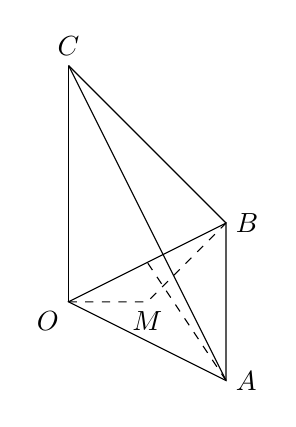
\begin{tikzpicture}
\draw (0,0) -- (2, -1) node[right]{$A$} -- (2, 1) node[right]{$B$} -- cycle;
\draw[dashed] (0,0) -- (1,0) node[below]{$M$} -- (2,1);
\draw[dashed] (2,-1) -- (1,0.5);
\draw (0,3) node[above]{$C$} -- (0,0) node[below left]{$O$};
\draw (0,3) -- (2,-1);
\draw (0,3) -- (2,1);
\end{tikzpicture}
\end{center}

$\star$ (ii) は、サラスの公式を使うと一瞬だったり、、
\[
\left[ \begin{array}{ccc}
x_1 & y_1 & z_1 \\
x_2 & y_2 & z_2 \\
x_3 & y_3 & z_3
\end{array} \right]
=
\left[ \begin{array}{ccc}
l & m & n \\
m & n & l \\
n & l & m
\end{array} \right]
\]
\begin{align*}
V &= \frac{1}{6} \left| lnm + mln + nml - l^3 - n^3 - m^3 \right| \\
&= \frac{1}{6} (l^2+m^2+n^2) = \frac{1}{6} ((l+m+n)^2-2\cdot 0) = \frac{1}{6}
\end{align*}
※ $\left| lnm+mln+nml - l^3-m^3-n^3 \right| = (l+m+n)(l^2+m^2+n^2-lm-mn-nl)$ などを利用。

(iii) $L\left(\frac{m+n}{2}, \frac{n+l}{2}, \frac{l+m}{2}\right)$, $M\left(\frac{n+l}{2}, \frac{l+m}{2}, \frac{m+n}{2}\right)$, $N\left(\frac{l+m}{2}, \frac{m+n}{2}, \frac{n+l}{2}\right)$
$P\left(\frac{1}{2}, \frac{m}{2}, \frac{n}{2}\right)$, $Q\left(\frac{m}{2}, \frac{n}{2}, \frac{l}{2}\right)$, $R\left(\frac{n}{2}, \frac{l}{2}, \frac{m}{2}\right)$ だから、
$Y\left(\frac{l+m+n}{4}, \frac{l+m+n}{4}, \frac{l+m+n}{4}\right)$ とおけば
\[ \overline{KY}^2 = \left(\frac{m+n-l}{4}\right)^2 + \left(\frac{n+l-m}{4}\right)^2 + \left(\frac{l+m-n}{4}\right)^2 = \text{const} \]
($K$ は $L \sim Q$ の任意の点) となり、たしかに $L \sim R$ は $Y$ を中心とする球面上にある。終

\subsection*{第4問}
[解] $\frac{1}{2}$ の確率で1点増し、$\frac{1}{2}$ の確率で1点減る。

$n$ 回目までに奇数の目が出た回数 $X(n)$ 、$n$ 回目までに偶数の目が出た回数 $Y(n)$ とおくと $n \le 5$ の時、常に
\[ X(n)+2 > Y(n) \quad (\because X(n)+Y(n)=n) \]
がみたされていれば良い ($n=5$ では等号が成立しても良い)。このような場合の数は、右の図で、格子の上を通って A から B まで行く最短経路のうち $Y=X+2$ を通らないものと1対1対応している。

\begin{center}
\begin{tikzpicture}[scale=0.8]
\draw[->] (-1,0) -- (6,0) node[right] {$X$};
\draw[->] (0,-1) -- (0,5) node[above] {$Y$};
\draw[step=1cm,gray,very thin] (0,0) grid (5,4);
\draw[thick, domain=-1:3] plot (\x, {\x+2}) node[right] {$Y=X+2$};
\node at (0,0) [below left] {$A$};
\node at (4,1) [above right] {$B$};
\fill (5,0) circle (2pt) node[below right] {持ち点 7};
\fill (4,1) circle (2pt) node[below right] {5点};
\fill (3,2) circle (2pt) node[below right] {3点};
\end{tikzpicture}
\end{center}

7点 $\cdots$ 1通り \\
5点 $\cdots$ 5通り \\
3点 $\cdots$ 9通り \\
1点 $\cdots$ 5通り

だから、
5回振ることのできる確率は $\frac{20}{2^5} = \frac{5}{8}$ 終

得点の期待値は $\frac{1}{2^5} (7+25+27+5) = \underline{2 \text{点}}$ 終

\subsection*{第5問}
[解] $\{a_n\}$ を小さい順にならびかえた数列 $\{b_n\}$ とする。

(i) $b_1$ により場合分けする。$b_1 \ge 0$ の時は、$b_n$ が単調増加であることから (イ) が成立する。そこで、$b_1 < 0$ の時、(ロ) が成立することを示す。

$b_n > 0$ と仮定する。すると、$b_k \le 0 < b_{k+1}$ をみたす $k (1 \le k \le n-1)$ が存在する。
\[ b_1 < b_2 < \cdots < b_k \le 0 < b_{k+1} < \cdots < b_n \]
この時、$b_1$ と $b_n$ をとりだしてきて、$b_1-b_n$ 又は $b_n-b_1$ のいずれかが $S$ の要素だが、$b_1 < 0 < b_n$ より
\[ b_1 - b_n > b_1 \quad, \quad b_n - b_1 > b_n \]
となり、$b_n$ が単調増加であることに反し矛盾。以上から $b_n \le 0$ となり、したがって (ロ) が成立する。

以上から示された 終

(ii) (イ) が成り立つ時
$S$ の全要素が $0$ 以上だから、$b_k, b_j$ をとってきた時 ($j<k$)、
$b_j - b_k < 0$ は $S$ の要素となりえず、$b_k - b_j$ が $S$ の要素となる。
したがって
\[ b_2 - b_1 < b_3 - b_1 < \cdots < b_n - b_1 \ (n-1\text{コ}) \]
が全て $S$ の要素となる！！

$1^{\circ} \ b_1 > 0$ の時
\[ b_1 \le b_2 - b_1 < b_3 - b_1 < \cdots < b_n - b_1 < b_n \]
となり、
$b_2 - b_1 = b_1, \cdots, b_n - b_1 = b_{n-1}$ となるから、順に
\[ b_2 = 2b_1, \ b_3 = 3b_1, \ \cdots \ b_n = nb_1 \]
となり、たしかに数列 $\{b_n\}$ は初項 $b_1(>0)$、公差 $b_1$ の等差数列

$2^{\circ} \ b_1 = 0$ の時
$b_2 > b_1 = 0$ から、同じようにして
\[ (0 < ) b_3 - b_2 < b_4 - b_2 < \cdots < b_n - b_2 (< b_n) \]
が全て $S$ の要素で、
\[ b_3 - b_2 = b_2, \cdots, \ b_n - b_2 = b_{n-1} \]
となり、$2 \le i$ の時 $b_i = i b_2$、$b_1=0$ だから $\{b_n\}$ は初項 $0$、公差 $b_2$ の等差数列。

(ロ) が成り立つ時
(イ) と同じく、
\[ b_1 - b_n < b_2 - b_n < \cdots < b_{n-1} - b_n \]
が全て $S$ の要素だから、(イ) の場合と全く同様にして $\{b_n\}$ が等差数列であることが示される。

以上から、いずれの場合も $\{b_n\}$ は等差数列。$\{b_n\}$ は $\{a_n\}$ をならびかえたものだから、示された 終

\subsection*{第6問}
[解] $f(x)$ を $f$ などと略記する

\begin{flushright}
$\left[ \text{よく考えると、わざわざ (2) で } (A,B)=(1,3) \text{ を排除する必要なかったね…} \right]$
\end{flushright}

(1) $g(x), h(x)$ は整数係数だから、$g(0), h(0) \in \mathbb{Z} \cdots \text{①}$.
又、$f(0) = g(0)h(0)$ から $1 = g(0)h(0) \cdots \text{②}$
①, ②から $(g(0), h(0)) = (1, 1), (-1, -1)$ となるが、いずれの場合も $g(0) = h(0)$ となる 終

(2) 題意の時、対称性から $(g\text{の次数}) \le (h\text{の次数})$ とすると、
$(A, B) = (1, 3), (2, 2)$ のいずれかである。
前者の時、$f$ の最高次係数が $1$ なことと (1) から
$g(x) = \pm x \pm 1$ となるが、$f(\pm 1) \neq 0$ と因数定理から、$f(x) = g(x)h(x)$ に矛盾。
よって $(A, B) = (2, 2)$ に限られる。以下 $f(m), g(m) \in \mathbb{Z}$ ($m \in \mathbb{Z}$) に注意する。

\begin{cases}
g(1)h(1) = 1 \\
g(a)h(a) = 1 \\
g(b)h(b) = 1
\end{cases}
より、(1) と同じく $g(1)=h(1), g(a)=h(a), g(b)=h(b)$ である。
$g, h$ は共に2次式であることと、異なる3つの値で $g, h$ の値が一致することから、$g(x) = h(x)$ となる 終

(3) $g=h$ の時
\[ (g+1)(g-1) = x(x-a)(x-1)(x-b) \cdots \text{③} \]
たとえば $(a, b) = (-1, -2)$、$g(x) = x^2+x-1$ とすれば
\[ (g+1)(g-1) = x(x+1)(x+2)(x-1) \]
となって③をみたすから
$(a, b) = (-1, -2)$ が1例である。終

\end{document}
